
\documentclass[letterpaper,hide notes,xcolor={table,svgnames},pdftex,10pt]{beamer}
\def\showexamples{t}


%\usepackage[svgnames]{xcolor}

%% Demo talk
%\documentclass[letterpaper,notes=show]{beamer}

\usecolortheme{crane}
\setbeamertemplate{navigation symbols}{}

\usetheme{MyPittsburgh}
%\usetheme{Frankfurt}

%\usepackage{tipa}

\usepackage{hyperref}
\usepackage{graphicx,xspace}
\usepackage[normalem]{ulem}
\usepackage{multicol}
\usepackage{amsmath,amssymb,amsthm,graphicx,xspace}
\newcommand\SF[1]{$\bigstar$\footnote{SF: #1}}

\usepackage[default]{sourcesanspro}
\usepackage[T1]{fontenc}

\newcounter{tmpnumSlide}
\newcounter{tmpnumNote}

% old question code
%\newcommand\question[1]{{$\bigstar$ \small \onlySlide{2}{#1}}}
% \newcommand\nquestion[1]{\ifdefined \presentationonly \textcircled{?} \fi \note{\par{\Large \textbf{?}} #1}}
% \newcommand\nanswer[1]{\note{\par{\Large \textbf{A}} #1}}


 \newcommand\mnote[1]{%
   \addtocounter{tmpnumSlide}{1}
   \ifdefined\showcues {~\tiny\fbox{\arabic{tmpnumSlide}}}\fi
   \note{\setlength{\parskip}{1ex}\addtocounter{tmpnumNote}{1}\textbf{\Large \arabic{tmpnumNote}:} {#1\par}}}

\newcommand\mmnote[1]{\note{\setlength{\parskip}{1ex}#1\par}}

%\newcommand\mnote[2][]{\ifdefined\handoutwithnotes {~\tiny\fbox{#1}}\fi
% \note{\setlength{\parskip}{1ex}\textbf{\Large #1:} #2\par}}

%\newcommand\mnote[2][]{{\tiny\fbox{#1}} \note{\setlength{\parskip}{1ex}\textbf{\Large #1:} #2\par}}

\newcommand\mquestion[2]{{~\color{red}\fbox{?}}\note{\setlength{\parskip}{1ex}\par{\Large \textbf{?}} #1} \note{\setlength{\parskip}{1ex}\par{\Large \textbf{A}} #2\par}\ifdefined \presentationonly \pause \fi}

\newcommand\blackboard[1]{%
\ifdefined   \showblackboard
  {#1}
  \else {\begin{center} \fbox{\colorbox{blue!30}{%
         \begin{minipage}{.95\linewidth}%
           \hspace{\stretch{1}} Some space intentionally left blank; done at the blackboard.%
         \end{minipage}}}\end{center}}%
         \fi%
}



%\newcommand\q{\tikz \node[thick,color=black,shape=circle]{?};}
%\newcommand\q{\ifdefined \presentationonly \textcircled{?} \fi}

\usepackage{listings}
\lstset{%
  keywordstyle=\bfseries,
  aboveskip=15pt,
  belowskip=15pt,
  captionpos=b,
  identifierstyle=\ttfamily,
  escapeinside={(*@}{@*)},
  stringstyle=\ttfamiliy,
  frame=lines,
  numbers=left, basicstyle=\scriptsize, numberstyle=\tiny, stepnumber=0, numbersep=2pt}

\usepackage{siunitx}
\newcommand\sius[1]{\num[group-separator = {,}]{#1}\si{\micro\second}}
\newcommand\sims[1]{\num[group-separator = {,}]{#1}\si{\milli\second}}
\newcommand\sins[1]{\num[group-separator = {,}]{#1}\si{\nano\second}}
\sisetup{group-separator = {,}, group-digits = true}

%% -------------------- tikz --------------------
\usepackage{tikz}
\usetikzlibrary{positioning}
\usetikzlibrary{arrows,backgrounds,automata,decorations.shapes,decorations.pathmorphing,decorations.markings,decorations.text}

\tikzstyle{place}=[circle,draw=blue!50,fill=blue!20,thick, inner sep=0pt,minimum size=6mm]
\tikzstyle{transition}=[rectangle,draw=black!50,fill=black!20,thick, inner sep=0pt,minimum size=4mm]

\tikzstyle{block}=[rectangle,draw=black, thick, inner sep=5pt]
\tikzstyle{bullet}=[circle,draw=black, fill=black, thin, inner sep=2pt]

\tikzstyle{pre}=[<-,shorten <=1pt,>=stealth',semithick]
\tikzstyle{post}=[->,shorten >=1pt,>=stealth',semithick]
\tikzstyle{bi}=[<->,shorten >=1pt,shorten <=1pt, >=stealth',semithick]

\tikzstyle{mut}=[-,>=stealth',semithick]

\tikzstyle{treereset}=[dashed,->, shorten >=1pt,>=stealth',thin]

\usepackage{ifmtarg}
\usepackage{xifthen}
\makeatletter
% new counter to now which frame it is within the sequence
\newcounter{multiframecounter}
% initialize buffer for previously used frame title
\gdef\lastframetitle{\textit{undefined}}
% new environment for a multi-frame
\newenvironment{multiframe}[1][]{%
\ifthenelse{\isempty{#1}}{%
% if no frame title was set via optional parameter,
% only increase sequence counter by 1
\addtocounter{multiframecounter}{1}%
}{%
% new frame title has been provided, thus
% reset sequence counter to 1 and buffer frame title for later use
\setcounter{multiframecounter}{1}%
\gdef\lastframetitle{#1}%
}%
% start conventional frame environment and
% automatically set frame title followed by sequence counter
\begin{frame}%
\frametitle{\lastframetitle~{\normalfont(\arabic{multiframecounter})}}%
}{%
\end{frame}%
}
\makeatother

\makeatletter
\newdimen\tu@tmpa%
\newdimen\ydiffl%
\newdimen\xdiffl%
\newcommand\ydiff[2]{%
    \coordinate (tmpnamea) at (#1);%
    \coordinate (tmpnameb) at (#2);%
    \pgfextracty{\tu@tmpa}{\pgfpointanchor{tmpnamea}{center}}%
    \pgfextracty{\ydiffl}{\pgfpointanchor{tmpnameb}{center}}%
    \advance\ydiffl by -\tu@tmpa%
}
\newcommand\xdiff[2]{%
    \coordinate (tmpnamea) at (#1);%
    \coordinate (tmpnameb) at (#2);%
    \pgfextractx{\tu@tmpa}{\pgfpointanchor{tmpnamea}{center}}%
    \pgfextractx{\xdiffl}{\pgfpointanchor{tmpnameb}{center}}%
    \advance\xdiffl by -\tu@tmpa%
}
\makeatother
\newcommand{\copyrightbox}[3][r]{%
\begin{tikzpicture}%
\node[inner sep=0pt,minimum size=2em](ciimage){#2};
\usefont{OT1}{phv}{n}{n}\fontsize{4}{4}\selectfont
\ydiff{ciimage.south}{ciimage.north}
\xdiff{ciimage.west}{ciimage.east}
\ifthenelse{\equal{#1}{r}}{%
\node[inner sep=0pt,right=1ex of ciimage.south east,anchor=north west,rotate=90]%
{\raggedleft\color{black!50}\parbox{\the\ydiffl}{\raggedright{}#3}};%
}{%
\ifthenelse{\equal{#1}{l}}{%
\node[inner sep=0pt,right=1ex of ciimage.south west,anchor=south west,rotate=90]%
{\raggedleft\color{black!50}\parbox{\the\ydiffl}{\raggedright{}#3}};%
}{%
\node[inner sep=0pt,below=1ex of ciimage.south west,anchor=north west]%
{\raggedleft\color{black!50}\parbox{\the\xdiffl}{\raggedright{}#3}};%
}
}
\end{tikzpicture}
}


%% --------------------

%\usepackage[excludeor]{everyhook}
%\PushPreHook{par}{\setbox0=\lastbox\llap{MUH}}\box0}

%\vspace*{\stretch{1}

%\setbox0=\lastbox \llap{\textbullet\enskip}\box0}

\setlength{\parskip}{\fill}

\newcommand\noskips{\setlength{\parskip}{1ex}}
\newcommand\doskips{\setlength{\parskip}{\fill}}

\newcommand\xx{\par\vspace*{\stretch{1}}\par}
\newcommand\xxs{\par\vspace*{2ex}\par}
\newcommand\tuple[1]{\langle #1 \rangle}
\newcommand\code[1]{{\sf \footnotesize #1}}
\newcommand\ex[1]{\uline{Example:} \ifdefined \presentationonly \pause \fi
  \ifdefined\showexamples#1\xspace\else{\uline{\hspace*{2cm}}}\fi}

\newcommand\ceil[1]{\lceil #1 \rceil}


\AtBeginSection[]
{
   \begin{frame}
       \frametitle{Outline}
       \tableofcontents[currentsection]
   \end{frame}
}



\pgfdeclarelayer{edgelayer}
\pgfdeclarelayer{nodelayer}
\pgfsetlayers{edgelayer,nodelayer,main}

\tikzstyle{none}=[inner sep=0pt]
\tikzstyle{rn}=[circle,fill=Red,draw=Black,line width=0.8 pt]
\tikzstyle{gn}=[circle,fill=Lime,draw=Black,line width=0.8 pt]
\tikzstyle{yn}=[circle,fill=Yellow,draw=Black,line width=0.8 pt]
\tikzstyle{empty}=[circle,fill=White,draw=Black]
\tikzstyle{bw} = [rectangle, draw, fill=blue!20, 
    text width=4em, text centered, rounded corners, minimum height=2em]
    
    \newcommand{\CcNote}[1]{% longname
	This work is licensed under the \textit{Creative Commons #1 3.0 License}.%
}
\newcommand{\CcImageBy}[1]{%
	\includegraphics[scale=#1]{creative_commons/cc_by_30.pdf}%
}
\newcommand{\CcImageSa}[1]{%
	\includegraphics[scale=#1]{creative_commons/cc_sa_30.pdf}%
}
\newcommand{\CcImageNc}[1]{%
	\includegraphics[scale=#1]{creative_commons/cc_nc_30.pdf}%
}
\newcommand{\CcGroupBySa}[2]{% zoom, gap
	\CcImageBy{#1}\hspace*{#2}\CcImageNc{#1}\hspace*{#2}\CcImageSa{#1}%
}
\newcommand{\CcLongnameByNcSa}{Attribution-NonCommercial-ShareAlike}

\newenvironment{changemargin}[1]{% 
  \begin{list}{}{% 
    \setlength{\topsep}{0pt}% 
    \setlength{\leftmargin}{#1}% 
    \setlength{\rightmargin}{1em}
    \setlength{\listparindent}{\parindent}% 
    \setlength{\itemindent}{\parindent}% 
    \setlength{\parsep}{\parskip}% 
  }% 
  \item[]}{\end{list}} 




\title{Lecture 10 --- Normalization }

\author{Jeff Zarnett \\ \small \texttt{jzarnett@uwaterloo.ca}}
\institute{Department of Electrical and Computer Engineering \\
  University of Waterloo}
\date{\today}


\begin{document}

\begin{frame}
  \titlepage

 \end{frame}



\begin{frame}
\frametitle{Normalization}

So far, we learned the syntax to create tables, and how to turn modelling diagrams into tables. 

The modelling diagrams give us some guidance and tell us about wrong ways to represent the data.

We don't yet have enough guidance as to what is correct. 

If we do a good job the relation will be in a \textit{normal form}. Yes, \textit{a} normal form... there are several.

\end{frame}



\begin{frame}
\frametitle{Normalization Example}

Combine instructor (having the attributes id, name, department, salary) with department (having an id, faculty, budget).

Our combined table means one larger relation replaces two smaller ones.

This isn't total nonsense because instructors do have a relationship with a department, but is this a good way to model the data?

\end{frame}



\begin{frame}
\frametitle{Normalization Example}

Intuition might tell you no, but think about why. 

There are two instructors, say, Sedra and Smith, both members of department of electrical \& computer engineering. 

In both tuples there will be an entry for the budget of the department. 

The budget data is duplicated and risks becoming inconsistent.

\end{frame}

\begin{frame}
\frametitle{Normalization Example}

Our intuition may tell us this is bad, but we would like a way to express it formally. 

Informally the rule is that each value of department name corresponds to at most one budget. 

The formal description is a \alert{functional dependency}. 

It is written \textit{dept\_name} $\rightarrow$ \textit{budget}. 


\end{frame}



\begin{frame}
\frametitle{Functional Dependency}

If there is a schema that consists just of the attributes for department name and budget, then the department name attribute could be the primary key.

Combining instructor and department breaks this rule, because we have duplicate entries for department and therefore this can't work.

The functional dependency shows us that data is duplicated and that indicates that we need to split the combined relation in a process called \alert{decomposition}.

\end{frame}



\begin{frame}
\frametitle{Silly Example is Silly}

The previous example is very egregiously and obviously wrong, making it simple to identify that there is a problem. 

In reality, a database will have many more tables and it will be harder to find out what the functional dependencies are. 

There is an algorithm for that which will be covered soon enough.
\end{frame}



\begin{frame}
\frametitle{Decompose ALL THE THINGS!}

The relation is \textit{employee( ID, name, street, city, province, postalcode )}.

We can decompose this into two schemas: \textit{employee(ID, name), address(name, street, city, province, postcode)}. 

Does this work? 

No -- two employees could have the same name and that is likely in the real world, as some names are extremely popular. 

\end{frame}



\begin{frame}
\frametitle{Do It Properly At Least}

If instead of defining the address relation to be based on name, we could use the ID instead, and it would work. 

\textit{employee(ID, name), address(employeeID, street, city, province, postcode)}. 

This is an acceptable decomposition and we call it \alert{lossless} because no information is lost. 

\end{frame}


\begin{frame}
\frametitle{Do It Properly At Least}


The first attempt at this caused a loss of information.

If two employees have the same name, there is the possibility of confusion, so it is called a \alert{lossy} decomposition. 

We do not perform lossy decompositions.

\end{frame}


\begin{frame}
\frametitle{Atomic Domains and 1NF}

Our E-R model allows attributes to be non-atomic, that is to say, divisible. 

If a course code is ``ECE356'', that attribute is non-atomic because it can be divided into two parts, the ``ECE'' and ``356'' components. 

If the domain is indivisible units, e.g., an integer, it is atomic.

\end{frame}



\begin{frame}
\frametitle{1NF}

A relation $R$ is said to be in the \alert{first normal form} (abbreviated as 1NF) if the domain of all attributes of $R$ are atomic. 

If some attribute is not atomic, then we could subdivide it to put it into 1NF. 

Instead of course being ``ECE356'' we could split  it up into department ``ECE'' and number ``356''. 

The primary key could still be composed of those two elements, mind you.


\end{frame}



\begin{frame}
\frametitle{1NF and Varchar}

Does this mean that a string (varchar) attribute can never be atomic, as one may take a subset? 

No, what really matters is how they are used in the database. 

If the application logic requires breaking up the attribute for some reason, then it is non-atomic. 

Course ECE356 vs Employee ID AA1234.

\end{frame}



\begin{frame}
\frametitle{Set Valued Attributes}

More than this, though, we don't like set-valued attributes. 

We don't want the faculty tuple to have a very long varchar attribute called departments which then contains multiple elements, separated by spaces... 

For example, Engineering is a faculty, and the list of departments would be ECE, MME, SYDE, etc. 

\end{frame}



\begin{frame}
\frametitle{Decomposition with Functional Dependencies}

The schema that we create is supposed to model entities and their relationships in the real world. 

The real world understanding tells us information about how data should be modelled: students have a student ID number; the student ID number is unique. 

If the database does not represent that information in some way, we have done something wrong. 

The real world constraints may be represented as a key or as a functional dependency.

\end{frame}

\begin{frame}
\frametitle{Decomposition with Functional Dependencies}

The schema is just the data model, and we care if the data in the tables conforms to the constraints. 

If the data in the table meets all the real-world constraints, that instance of the relation is called a \alert{legal instance}. 

If all tables in the database are a legal instance of that relation, then we can say the instance of the database is a legal instance of the database schema.

\end{frame}



\begin{frame}
\frametitle{Supergir... Superkey!}

A \alert{superkey} is a subset $K$ of a relation $R$ if, in any legal instance of $R$, for all pairs, of tuples $t_{1}$ and $t_{2}$ in the instance of $r$, if $t_{1} \neq t_{2}$ then $t_{1}[K] \neq t_{2}[K]$. 

This is to say that no two tuples in a legal instance of the relation may have the same values the subset of attributes $K$.

Or if you prefer, the attributes in $K$ allow a tuple in the relation to be uniquely identified.

\end{frame}


\begin{frame}
\frametitle{Superkey}

Suppose that attributes $\alpha$ and $\beta$ are part of a relation $r$. 

A functional dependency $\alpha \rightarrow \beta$ is satisfied if for all pairs of tuples $t_{1}$ and $t_{2}$ such that $t_{1}[\alpha] = t_{2}[\alpha]$ it is the case that $t_{1}[\beta] = t_{2}[\beta]$. 

If this functional dependency holds on every legal instance of the relation, we can say the functional dependency holds on the schema.

\end{frame}



\begin{frame}
\frametitle{Superkey}

We can say that $K$ is a superkey of $R$ if the functional dependency $K \rightarrow R$ holds on this instance of the relation. 

That means, formally, that if $t_{1}[K] = t_{2}[K]$ then it means $t_{1} = t_{2}$ because a superkey identifies a tuple uniquely.


\end{frame}



\begin{frame}
\frametitle{Use of Functional Dependencies}

Functional dependencies are used for both design and verification purposes. 

We use them in the design process to identify and record the constraints that our database schema should be designed around. 

They will be used as a way to decide what entities should be formed and how their relationships to others appear. 

And when we have a set of functional dependencies, we can use them to verify if an instance of the database is legal.

If the answer is yes, then we say the set of functional dependencies holds.

\end{frame}


\begin{frame}
\frametitle{Use of Functional Dependencies}

\begin{center}
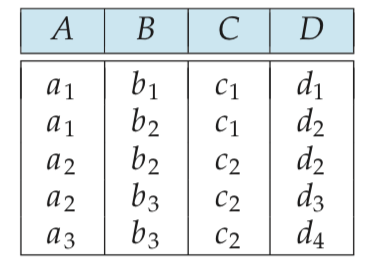
\includegraphics[width=0.5\textwidth]{images/fd-1}
\end{center}

What can we observe in this data?

\end{frame}



\begin{frame}
\frametitle{Trivial Functional Dependencies}

There are also \alert{trivial} functional dependencies because they are always true.

The functional dependency $A \rightarrow A$ is an example of a trivial dependency. 

A formal definition of a trivial relation is that $\alpha \rightarrow \beta$ is trivial if $\beta$ is a contained within $\alpha$ (in set thinking).

\end{frame}


\begin{frame}
\frametitle{Transitive Functional Dependencies}

Functional dependencies can be transitive: if $A \rightarrow B$ and $B \rightarrow C$, then $A \rightarrow C$. 

For each $A$ there can be only one value of $B$ and for that value of $B$ there is only one corresponding $C$. 

If a set of functional dependencies is $F$, the notation that includes all of these implied dependencies is $F^{+}$, the \textit{closure} of $F$.


\end{frame}



\begin{frame}
\frametitle{BCNF}

The \alert{Boyce-Codd Normal Form}, known as BCNF, eliminates all redundancy that can be found using functional dependencies.

A schema $R$ is in BCNF with respect to a set of functional dependencies in $F$, if, for all functional dependencies in $F^{+}$ of the form $\alpha \rightarrow \beta$ either: \\
\quad (1) the functional dependency is trivial, or\\
\quad (2) $\alpha$ is a superkey for schema $R$.


\end{frame}


\begin{frame}
\frametitle{Example Callback}
Calling back to the earlier example where we looked at merging instructor and relation, we can see that this is not in BCNF fairly easily. 

In this relationship a the department name is not a superkey because we had two entries (Sedra, Smith) that were in the same department 

Those had the same budget. A department cannot have two budgets.

There should exist a functional dependency. Check it against BCNF conditions.

\end{frame}


\begin{frame}
\frametitle{BCNF Decomposition}

If it is not in BCNF there is at least one nontrivial functional dependency $\alpha \rightarrow \beta$ where $\alpha$ is not a superkey for $R$. 

Then we need to split up $R$ into two relations: (1) $(\alpha \cup \beta)$ and (2) $(R - (\beta - \alpha))$. 


We may need to repeat that process on 1 of the new relations until it is in BCNF.


\end{frame}



\begin{frame}
\frametitle{Dependency Preservation}

 Avoiding duplication of data is not our only goal in a database design. 
 
 Constraints also need to be checked. 
 
Joins are expensive and we would like to avoid them. 
 
 Checking if a constraint is satisfied may require a computationally expensive join if the relations are in BCNF.


\end{frame}



\begin{frame}
\frametitle{BCNF Example}

\begin{center}
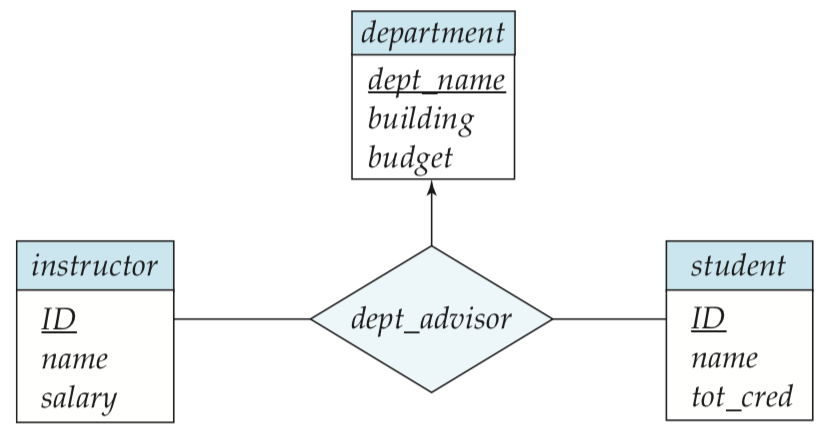
\includegraphics[width=0.8\textwidth]{images/advise-3}
\end{center}

The functional dependencies are \textit{instructor\_id} $\rightarrow$ \textit{dept\_name} (an instructor belongs to one department), and \textit{student\_id, dept\_name} $\rightarrow$ \textit{instructor\_id}.


\end{frame}



\begin{frame}
\frametitle{BCNF Example}

This design is not in BCNF, because \textit{instructor\_id} is not a superkey.

An instructor ID alone is not enough to identify the relationship, because multiple students can be advised by the same individual. 

So we need to perform the decomposition procedure and that will produce two relations: \textit{(student\_id, instructor\_id)} and \textit{(instructor\_id, dept\_name)}.

\end{frame}



\begin{frame}
\frametitle{BCNF Example}

It is difficult to verify the constraint that requires us to verify that each triple of \textit{(student\_id, instructor\_id, dept\_name}) is unique. 

That is because performing this check requires a join on the two relations. 

Because it is now hard to check this dependency, the design is said to not be \alert{dependency preserving}. 

Data is not lost, just harder to check and verify.

\end{frame}

\begin{frame}
\frametitle{2NF and 3NF}

The Third Normal Form, or 3NF, is weaker than BCNF that allows dependencies to be preserved. 

Is BCNF the second normal form? No, it is separate from BCNF. 

A table is in the second normal form if it is in the first normal form and all non-key columns are dependent on the table's primary key.

\end{frame}



\begin{frame}
\frametitle{3NF}

The 3NF rules are a small modification of the BCNF rules. 

In particular, we would like to allow some nontrivial functional dependencies whose left side (the $\alpha$) is not a superkey. 

\end{frame}


\begin{frame}
\frametitle{3NF Formally}
A schema $R$ is in 3NF with respect to a set of functional dependencies in $F$, if, for all functional dependencies in $F^{+}$ of the form $\alpha \rightarrow \beta$ one of the following holds: 

(1) the functional dependency is trivial, or 

(2) $\alpha$ is a superkey for schema $R$, or 

(3) Each attribute $A$ in $\beta - \alpha$ is contained in a candidate key for $R$.

\end{frame}



\begin{frame}
\frametitle{BCNF vs 3NF}

Remember that a schema that is in BCNF would satisfy case 1 or 2 for each of the functional dependencies, so anything in BCNF is already in 3NF. 

3NF, however, is slightly less restrictive and allows functional dependencies that are not permitted in BCNF, so something in 3NF may or may not be in BCNF.

\end{frame}



\begin{frame}
\frametitle{Example in 3NF}

The relation in the diagram in the previous subsection to represent \textit{dept\_advisor} contains three attributes. 

All primary keys in the other relations: \textit{(student\_id, instructor\_id, dept\_name)}. 

Based on what we know of the functional dependencies, this is already in 3NF. 

The step we took to do the decomposition to BCNF is unnecessary here if we can accept 3NF.

How do we know the new definition of \textit{dept\_advisor} is in 3NF?

\end{frame}



\begin{frame}
\frametitle{Higher Normal Forms}

This isn't even my final form! In addition to the first, second, third, and BCNF normal forms there are more... Fourth, fifth, and beyond.  

The fourth normal form is built upon the third normal form, so the first requirement for something being in 4NF is that it is in BCNF. 

The new requirement is that a record type cannot have more than one multivalued dependency.

\end{frame}



\begin{frame}
\frametitle{Higher Normal Forms}

A multivalued dependency exists between two attributes if, for each value of the first attribute $\alpha$ there is more than one value of the second attribute $\beta$.

Consider the following table representing students. It lists their department and their research areas. 

\begin{center}
\begin{tabular}{|l|l|l|} \hline
	\textbf{id} & \textbf{department} & \textbf{research\_area} \\ \hline
	20000001 & ECE & Security \\ \hline
	20000002 & CS & Software \\ \hline
    20000003 & ECE & Circuits \\ \hline
    20000004 & SYDE & HCI \\ \hline
    20000005 & ECE & Networks \\ \hline
    20000005 & CS & Security \\ \hline
\end{tabular}
\end{center}

\end{frame}



\begin{frame}
\frametitle{4NF Decomposition Algorithm}

The formal 4NF decomposition algorithm looks something like this:

\begin{enumerate}
	\item Compute $D^{+}$
	\item Check all relations to see if they are in 4NF.
	\item If all relations are in 4NF with respect to the constraints, the algorithm terminates.
	\item Otherwise let $\alpha \rightarrow\rightarrow \beta$ be a multivalued dependency in the relation $R_{i}$ that has two or more multivalued dependencies. 
	\item Split the relation into two new ones, $(R_{i} - \beta)$ and $(\alpha, \beta)$.
	\item Go back to step 2.
\end{enumerate}

\end{frame}



\begin{frame}
\frametitle{Fifth Normal Form}

The fifth normal form, as described in the MariaDB documentation, is one where you can't make tables any smaller with different keys. 

People have also tried to design sixth normal forms... 

There's some talk in the literature about domain key normal form but these are mostly of theoretical or academic research interest only.

So we will focus on BCNF and 3NF mostly.

\end{frame}





\end{document}

